The software of \US\ is divided into several modules. 'Module' is a common name for apps and libraries.The \US\ application is the main module. It cannot work alone but relies on other, so-called \concept{plug-in} libraries. When you install \US, it comes with a standard repertoire of plug-in libraries. All the box classes, that you use to build models in box scripts, are defined in such plug-ins. To add you own box classes to represent starfish, lice, palm trees or whatever, you code your own plug-in. The box classes that you code in your own plug-in (or more plug-ins) will be available for model-building on par with the standard plug-ins. You can also make your plug-ins available to other modellers.

\section{Download \protect\US\ source code}
To code you own plug-in, you need to get used to a certain workflow. You will benefit from downloading the latest version of the \US\ source code quite frequently, as \US\ is undergoing rapid development. You can find the source code at \url{https://github.com/NielsHolst/UniSim2/releases}. Click the \gui{zip} button of the latest release.

You should keep a tidy computer not to get source code versions mixed up. Each \US\ version resides in a single folder labelled by the version number(\iref{fig:unisim-versions}). Keep the different versions inside one parent folder, traditionally called \filename{dev}. Whenever you download the latest \US\ source code, unpack it in the \filename{dev} folder.

\US\ source code comes in a zip file with just one item inside, a folder named \filename{UniSim2-2.\em{m.n}}, where \filename{\em{m}} and \filename{\em{n}} are running version numbers. With repeated downloads your \filename{dev} folder will start to fill up with \US\ source of progressing versions (\iref{fig:unisim-versions}). Once in a while you may want to delete folders with older versions.

If you are an experienced programmer, you may prefer to use the git version control system. If so, you git-clone the project once and then keep it updated with git-pull.

\begin {figure} [ht]
\centering
\tikzstyle{every node}=[draw=black,anchor=west]
\begin{tikzpicture}[%
  grow via three points={one child at (0.5,-0.7) and
  two children at (0.5,-0.7) and (0.5,-1.4)},
  edge from parent path={(\tikzparentnode.south) |- (\tikzchildnode.west)}]
  \node {dev}
   child {node {boost}}
   child {node {UniSim2-2.0.10}}
   child {node {UniSim2-2.0.11}}
   child {node {UniSim2-2.0.14}}
 ;
\end{tikzpicture}
\caption{Layout of \US\ source code folders of different versions inside the \filename{dev} folder. You always work inside the most recent (version 2.0.14 in this case). The same \filename{boost} library (\iref{ch:install-boost}) is used by all versions. Create the \filename{dev} folder so that its path contains no spaces: \filename{C:/dev} or \filename{\mytilde/dev} are fine, but \filename{C:/users/John Smith/dev} is not. The \devhome\ symbol is used as a shorthand for the \filename{dev} folder.}
\label{fig:unisim-versions}
\end{figure}

You will avoid much confusion by keeping your \filename{dev} folder clean always, as exemplified in \iref{fig:unisim-versions}. The \filename{dev} folder itself contains nothing but sub-folders.

\section{Build \protect\US}
Turning \CPP\ source code into an app and its libraries involves two steps: compile and link. They are usually considered as one step: build, which is also known as 'make'. Programmers in a hurry will mix these terms, and you will hear the words 'compile', 'build' and 'make' interchangeably.

Information about which \CPP\ files make up the source for a certain app and its libraries are kept in a \concept{project} file. For \US\ you find this file easily in the source code folder, \eg\ in \filename{dev/UniSim2-2.0.14}. The project file always has the same name, regardless of the version. It is \filename{UniSim2.pro}.

Qt Creator is the tool we use, both for writing the \CPP\ source and for for building \US. The build system is intelligent. So if you change only a single file then only that file and module will be rebuild. This is important because building the whole \US\ source code is time-consuming. Maybe 5 minutes.

\begin{figure}
\centering
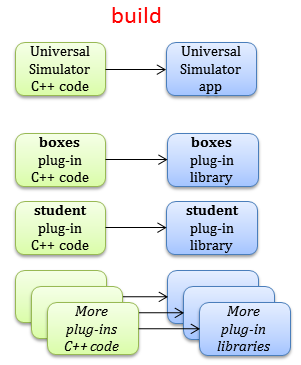
\includegraphics[scale=0.8]{graphics/workflow-build}
\caption{Building the \US\ app and plug-in libraries from source.}
\label{fig:workflow-build}
\end{figure}

The build process produces one or more files for each module. The exact file names vary a little between operating systems. The app itself will be named \filename{unisimd} and placed in the binaries folder (\filename{\devhome/UniSim2/bin}). 

The \US\ base library is compiled into \filename{libuniversal_simulator_based}. On Windows, it is placed in the binaries folder together with the app. On Mac OS X, it is placed in the \filename{\mytilde/lib} folder. Caveat: The \filename{\mytilde/lib} folder must be writable. Otherwise, Qt Creator will stop with an error, when it tries to write the base library file.

The plug-in binaries are all put in the \filename{\devhome/UniSim2/bin/plugins} folder. If you are ever in doubt which modules you just built, you can check the time stamp of these binary files.

Whenever you have downloaded the latest \US\ source code, your first step is to build it in Qt Creator. Only then do you proceed with your own plug-in development. You build the project by opening the \filename{UniSim2} project file in Qt Creator. Accept, if Qt Creator suggests you should configure your project. Then you click Build in the Build menu. When you've got a green bar in the lower right corner, you are done.

\section{Update the source code version}
You should get used to the procedure for updating the \US\ source code. The problem that you need to resolve every time is to merge your own code (programmed in a previous version, let's say 2.0.14) with that of \US\ itself in a newer version (let's say 2.0.17). The merging is straightforward because you are coding only inside your own plug-in, and the \CPP\ code for each plug-in is located inside its own folder.

For a quick start with \US\ programming, you have maybe added code to the \concept{student} plug-in, which comes as part of the \US\ source code. You can keep on adding code to this plug-in considering it your own. However, when at some point you want to make your plug-in available to others, you will need to rename it and give at a unique name (\todo{instructions to follow}).

If you are a programmer, you may know how to use the git version control system. If so git-pull is all you need to update and merge you source code. Otherwise, it is not too difficult. Let's say you have added additional boxes to the student plug-in located in \filename{\devhome/UniSim-2.0.14/src/plugins/student}. Then you download the latest source code which happens to be version 2.0.17. These are the steps you should follow to merge the code:
\begin{enumerate}
\item In Qt Creator close all projects and files. This can be achieved in a single step from the File menu.
\item In Qt Creator open the \filename{UniSim2.pro} file of the newest version (\ie\ \filename{\devhome/UniSim-2.0.17/UniSim2.pro}).
\item Build the project. Proceed only when you have gotten a green bar.
\item Copy the source code of your plug-in from the older version to the new version:
\begin{enumerate}
\item Using your preferred file management software (\eg\ File Explorer or Finder), navigate to the plug-ins source code folder in the older version (\eg\ \filename{\devhome/UniSim-2.0.14/src/plugins}).
\item Copy the \filename{student} folder found there (\eg\ \filename{\devhome/UniSim-2.0.14}\\\filename{/src/plugins/student}).
\item Navigate to the \filename{plugins} source code folder in the newest version (\eg\ \filename{\devhome/UniSm-2.0.17/src/plugins}).
\item Paste the \filename{student} folder there, overwriting the present \filename{student} folder (\eg\ \filename{\devhome/UniSim-2.0.17/src/plugins/student}).
\end{enumerate}
\item Back in Qt Creator you still have the newest \US\ project file open; else open it (\filename{\devhome/UniSim-2.0.17/UniSim2.pro}).
\item Build the project. You should get a green bar.
\item If you get a red bar:
\begin{enumerate}
\item Your code likely had errors even before you began the whole update procedure. Verify this by closing the project (2.0.17) and re-opening the previous project (2.0.14). Build the previous project to verify that your code was indeed faulty. Fix the error and proceed only on a green bar.
\item In the unlikely event that your code builds under the previous version (2.0.14) but not under the new (2.0.17), zip your plug-in source code (\ie\ in this example, \filename{\devhome/UniSim2-2.0.14/src/plugins/student}) and send it to \USS.
\end{enumerate}
\end{enumerate}

After you have completed merging your code into the newest version you just continue working in that version, \ie\ in this example continue with the project in \filename{\devhome/UniSim2-2.0.17}.

Note that your box scripts remain untouched by the update procedure above, as long as you keep them outside the \US\ source folders (\filename{\devhome/UniSim2-2.\em{m.n}}). Hint: Your box scripts most likely are in their default location at \filenameexplained{input}.

\section{Run \protect\US}
When the app and its libraries have been built, the app is ready for execution (also called 'launching'). You can either run the app from within Qt Creator (by way of the Build menu or by clicking the green triangle in the lower left corner), or you can double-click the \US\ app file (found in \filename{\devhome/UniSim2/bin}) in File Explorer (Windows), Finder (OS X) or similar navigation software. The second option launches quicker but in Windows it only works, if you have put the Qt libraries on the system path as described in \iref{ch:build-us}.

\section{Inside \protect\US}
When you \uscom{load} a box script at the \US\ prompt, \US\ will search its plug-ins to find the box classes you refer to in the box script, \eg\ \code{Stage} and \code{Records}. If you have defined, \eg\ a \code{Tomato} class in your own plug-in, then \US\ will find that too; if you load a box script that uses the \code{Tomato} class.

In response to the \uscom{run} command, \US\ will carry out the \code{run} method of the outermost class in the box script (usually, a \code{Simulation} box), which effectuates the computation steps as explained in \iref{ch:computations}.

The \code{OutputR} box, usually present as the last box in a box script, produces output in the form of two files (\filename{.txt} and \filename{.R}) and a snippet of R code copied to the clipboard, which you can subsquently paste into the R program to study the simulation output (see \iref{ch:view-model-output}).


\begin{figure}
\centering
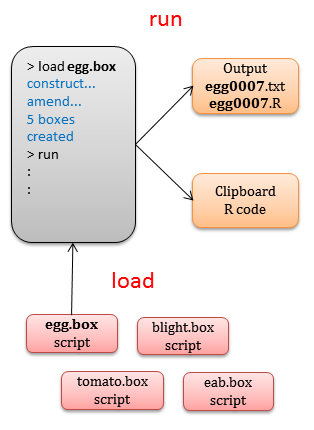
\includegraphics[scale=0.8]{graphics/workflow-execute}
\caption{Executing the \US\ app.}
\label{fig:workflow-execute}
\end{figure}

